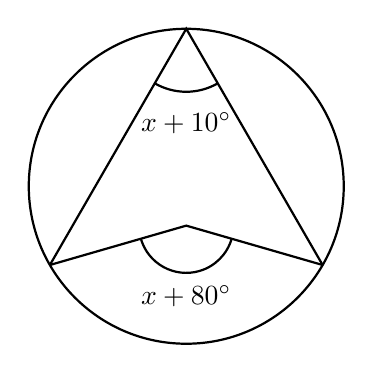
\begin{tikzpicture}[scale=1]

    % Define center of the circle
    \coordinate (O) at (0,0);
    
    % Draw the circle
    \draw[thick] (O) circle (2cm);
    
    % Define points on the circle
    \coordinate (A) at (0, 2); % Top point
    \coordinate (B) at (-1.732, -1); % Bottom left point
    \coordinate (C) at (1.732, -1); % Bottom right point
    \coordinate (D) at (0, -0.5); % Center inner point

    % Draw lines connecting points
    \draw[thick] (B) -- (A) -- (C);
    \draw[thick] (B) -- (D) -- (C);

    % Draw arc for angle x+10
    % Angle from A to B is exactly 240 degrees, and A to C is exactly 300 degrees.
    % We use the relative coordinate addition '++(angle:radius)' to ensure the arc starts exactly on the line AB.
    \draw[thick] (A) ++(240:0.8) arc (240:300:0.8);
    \node at (0, 0.8) {$x+10^{\circ}$};

    % Draw arc for angle x+80
    % The vector from D(0, -0.5) to B(-1.732, -1) has an angle of approx 196.1 degrees.
    % The vector from D(0, -0.5) to C(1.732, -1) has an angle of approx 343.9 degrees.
    \draw[thick] (D) ++(196.1:0.6) arc (196.1:343.9:0.6);
    \node at (0, -1.4) {$x+80^{\circ}$};

\end{tikzpicture}